%File: anonymous-submission-latex-2024.tex
\documentclass[letterpaper]{article} % DO NOT CHANGE THIS
\usepackage[submission]{aaai24}  % DO NOT CHANGE THIS --[submission] will remove the NAME
\usepackage{times}  % DO NOT CHANGE THIS
\usepackage{helvet}  % DO NOT CHANGE THIS
\usepackage{courier}  % DO NOT CHANGE THIS
\usepackage[hyphens]{url}  % DO NOT CHANGE THIS
\usepackage{graphicx} % DO NOT CHANGE THIS
\urlstyle{rm} % DO NOT CHANGE THIS
\def\UrlFont{\rm}  % DO NOT CHANGE THIS
\usepackage{natbib}  % DO NOT CHANGE THIS AND DO NOT ADD ANY OPTIONS TO IT
\usepackage{caption} % DO NOT CHANGE THIS AND DO NOT ADD ANY OPTIONS TO IT
\frenchspacing  % DO NOT CHANGE THIS
\setlength{\pdfpagewidth}{8.5in} % DO NOT CHANGE THIS
\setlength{\pdfpageheight}{11in} % DO NOT CHANGE THIS
%
% These are recommended to typeset algorithms but not required. See the subsubsection on algorithms. Remove them if you don't have algorithms in your paper.
\usepackage{algorithm}
\usepackage{algorithmic}

\usepackage{booktabs} % 用于绘制高质量的三线表
\usepackage{graphicx} % 可能用于图形或调整大小
\usepackage{tabularx}

%
% These are are recommended to typeset listings but not required. See the subsubsection on listing. Remove this block if you don't have listings in your paper.
\usepackage{newfloat}
\usepackage{listings}
\DeclareCaptionStyle{ruled}{labelfont=normalfont,labelsep=colon,strut=off} % DO NOT CHANGE THIS
\lstset{%
	basicstyle={\footnotesize\ttfamily},% footnotesize acceptable for monospace
	numbers=left,numberstyle=\footnotesize,xleftmargin=2em,% show line numbers, remove this entire line if you don't want the numbers.
	aboveskip=0pt,belowskip=0pt,%
	showstringspaces=false,tabsize=2,breaklines=true}
\floatstyle{ruled}
\newfloat{listing}{tb}{lst}{}
\floatname{listing}{Listing}
%
% Keep the \pdfinfo as shown here. There's no need
% for you to add the /Title and /Author tags.
\pdfinfo{
	/TemplateVersion (2024.1)
}
\title{Report for AI6127 Assignment 1}
\author{
	Zhang Yu
}

%\affiliations{\part{title}
	%	Nanyang Technological University
	%}

\begin{document}
	
\maketitle 

\section{The influence of different optimizers on classification performance}

In this text sentiment analysis experiment using the IMDB dataset, an RNN with 256 hidden states was used, and the embedding dimension for the text was set to 100. To investigate the impact of different optimizers (SGD, Adam, AdaGrad) on classification performance, the model was trained for the same number of epochs while keeping the training dataset and network structure unchanged. The learning rate used for training was 0.001, and the batch size was set to 64.

When the training epoch is set to 20, the classification performance obtained by the model is shown in the table below (Table 1). The results show that the model using the Adam optimizer achieved the best classification performance, with an accuracy of 72.35\% on the test set. The model using AdaGrad also achieved good results, with an accuracy of 71.54\%. However, the model using SGD optimizer did not exhibit performance significantly better than random guessing. Considering that this phenomenon might be caused by underfitting, a new training experiment with 200 epochs was conducted.

\begin{table}[H] % [t] 倾向于将表格放在栏目的顶部
	\centering % 使表格在当前栏目中居中
	\caption{Performance with different optimizers (20 epochs)} 
	\label{tab:various optimizers} 	
	% 表格的实际内容：四列，分别为左对齐(l)、居中(c)、居中(c)、居中(c)
	\begin{tabularx}{\columnwidth}{l X X X X}
		\toprule 
		\textbf{Optimizer} & \textbf{Val.Loss} & \textbf{Val.Accu} & \textbf{Test.Loss} & \textbf{Test.Accu} \\ 
		\midrule 
		SGD & 0.685 & 54.66\% & 0.685 & 54.74\%\\
		Adam & 0.659 & 76.98\% & 0.563 & 72.35\%\\
		AdaGrad & 0.566 & 71.39\% & 0.567 & 71.54\% \\
		\bottomrule 
	\end{tabularx}
\end{table}

The results after 200 epochs of training are shown in the table below (Table 2). It can be observed that the performance of the model using Adam did not significantly improve on the test set, while the model using AdaGrad showed a slight improvement and surpassed Adam's performance. Furthermore, the classification accuracy of the model using SGD notably increased, but it still did not exceed the performance of the other two optimizers.

\begin{table}[H] % [t] 倾向于将表格放在栏目的顶部
	\centering % 使表格在当前栏目中居中
	\caption{Performance with different optimizers (200 epochs)} 
	\label{tab:various optimizers 2} 	
	% 表格的实际内容：四列，分别为左对齐(l)、居中(c)、居中(c)、居中(c)
	\begin{tabularx}{\columnwidth}{l X X X X}
		\toprule 
		\textbf{Optimizer} & \textbf{Val.Loss} & \textbf{Val.Accu} & \textbf{Test.Loss} & \textbf{Test.Accu} \\ 
		\midrule 
		SGD & 0.611  & 67.39\% & 0.603 & 68.24\%\\
		Adam & 1.691 & 70.18\% & 0.610 & 72.52\%\\
		AdaGrad & 0.558  & 74.92\% & 0.565 & 74.46\% \\
		\bottomrule 
	\end{tabularx}
\end{table}

By plotting the training loss (Figure 1) and validation accuracy (Figure 2) throughout the model training process, the optimization performance of the three different optimizers can be better compared. Based on the results from both experiments, the convergence speed of Adam and AdaGrad is noticeably faster than that of SGD. Adam is the fastest among the three, achieving a significant optimization effect after approximately 20 epochs, and its training loss decreased at a rate faster than the other two optimizers during training. What also should be noted is that during the training process, the AdaGrad optimizer showed less fluctuation in both the training loss and the validation set accuracy compared to the other two optimizers.


 
\begin{figure}[H] 
	\centering 
	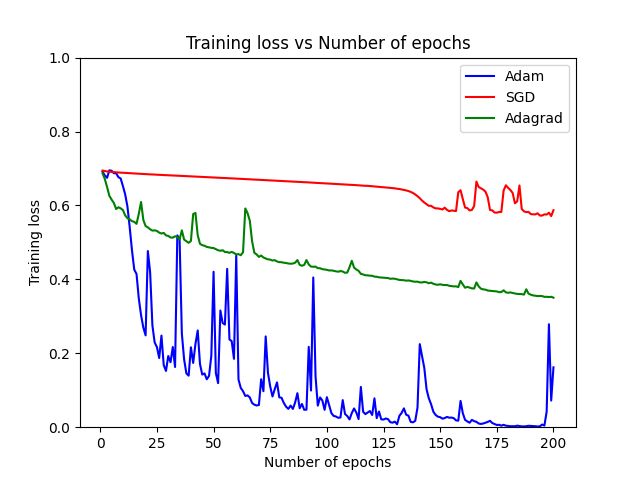
\includegraphics[width=0.45\textwidth]{Performance with different optimizers (200 epochs)_ Train loss.png}  
	\caption{Training loss with different optimizers} 
	\label{Fig.1} 
\end{figure}

\begin{figure}[H] 
	\centering 
	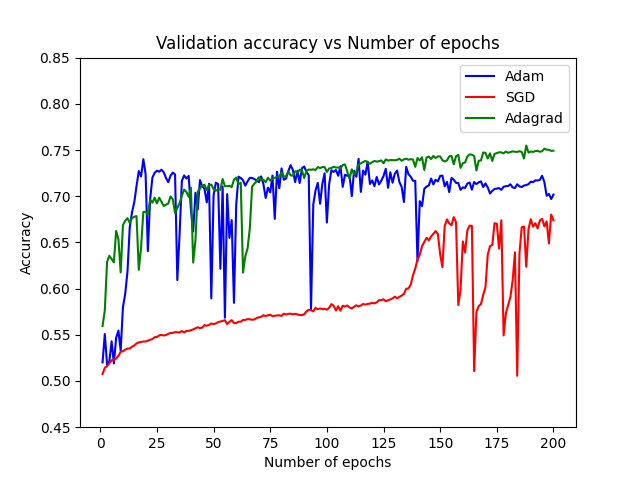
\includegraphics[width=0.45\textwidth]{Performance with different optimizers (200 epochs)_ val acc}  
	\caption{Validation accuracy with different optimizers} 
	\label{Fig.2} 
\end{figure}

The reason for the above phenomenon is the different strategies used by the three optimizers when updating weights. As discussed in \cite{kingma2014adam}, AdaGrad and Adam efficiently handle sparse features because they provide a larger, adaptive learning rate for sparse gradients. SGD, in comparison, is notably slow at learning these features, which explains the faster convergence of the former two optimizers.

The reason why AdaGrad becomes more stable in the later stages of training can also be found in its weight update strategy (Equation 1-2): it uses the sum of all historical squared gradients to obtain $G_{t, ii}$. This causes the denominator of the learning rate to continuously increase, thereby causing the final learning rate to become extremely small. Adam, in contrast, replaces AdaGrad's pure accumulation with an exponential moving average (Equation 3-5) to ensure that the denominator of the learning rate only reflects the recent variance of the gradients, rather than the sum of the entire training history. This improvement in Adam prevents premature learning rate decay.

\begin{equation}
	\theta_{t+1, i} = \theta_{t, i} - \frac{\eta}{\sqrt{G_{t, ii} + \epsilon}} \cdot g_{t, i}
\end{equation}

\begin{equation}
	G_{t, ii} = \sum_{\tau=1}^{t} g_{\tau, i}^2
\end{equation}

\begin{equation}
	\theta_{t+1} = \theta_t - \frac{\eta}{\sqrt{\hat{v}_t} + \epsilon} \cdot \hat{m}_t
\end{equation}

\begin{equation}
	\hat{m}_t = \frac{m_t}{1 - \beta_1^t}
\end{equation}

\begin{equation}
	\hat{v}_t = \frac{v_t}{1 - \beta_2^t}
\end{equation}


\section{The influence of different epoch settings on classification performance}

In this section, the same RNN model as in the first section was used for the text sentiment classification task, with the optimizer fixed to Adam, and training was performed across four different epoch settings. The experimental results are shown in the table below (Table 3).


\begin{table}[H] % [t] 倾向于将表格放在栏目的顶部
	\centering % 使表格在当前栏目中居中
	\caption{Performance with different epochs} 
	\label{tab:various epoch} 	
	% 表格的实际内容：四列，分别为左对齐(l)、居中(c)、居中(c)、居中(c)
	\begin{tabularx}{\columnwidth}{l X X X X}
		\toprule 
		\textbf{Epoch} & \textbf{Val.Loss} & \textbf{Val.Accu} & \textbf{Test.Loss} & \textbf{Test.Accu} \\ 
		\midrule 
		5 & 0.692 & 52.22\% & 0.647 & 61.83\%\\
		10 & 0.668 & 55.51\% & 0.658 & 62.13\%\\
		20 & 0.659 & 76.98\% & 0.563 & 72.35\% \\
		50 & 0.896 & 75.79\% & 0.594 & 71.41\% \\
		\bottomrule 
	\end{tabularx}
\end{table}

The experimental results show that as the epoch count increased from 5 to 20, the classification performance gradually improved. However, when the epoch count was further increased to 50, the model's performance did not show a significant improvement and even slightly declined.

By combining the results of this section's experiment with the model performance graph (Figure 1 and 2) from the first section, it can be concluded that before 20 epochs, the model was likely underfitting, which is why performance gradually improved as the number of epochs increased. However, after 20 epochs, although the training loss continued to decrease, the accuracy on both the validation and test sets declined. At this point, the model may have gradually started to overfit, and continuing to increase the number of epochs will not result in an improved model.

Another possible reason for the model's performance failing to improve after 20 epochs could be the limitations of Adam. As seen from the training graphs, Adam's performance fluctuates significantly as epochs increase. This behavior can be attributed to the instability of Adam's adaptive learning rate. Near a local minimum, the estimate of the $v_t$ can become very small, causing the optimizer to take an excessively large step. This results in overshooting, which prevents the training loss from converging to a stable lower value \cite{reddi2019convergence}.
	
\section{The influence of different models on classification performance}

In this section, several different models were used to experiment with their performance on the sentiment classification task. All models utilized the Adam optimizer and were trained for 50 epochs. The training results are shown in the table below (Table 4).

\begin{table}[H] % [t] 倾向于将表格放在栏目的顶部
	\centering % 使表格在当前栏目中居中
	\caption{Performance with different models} 
	\label{tab:various model} 	
	% 表格的实际内容：四列，分别为左对齐(l)、居中(c)、居中(c)、居中(c)
	\begin{tabularx}{\columnwidth}{l X X X X}
		\toprule 
		\textbf{Model} & \textbf{Val.Loss} & \textbf{Val.Accu} & \textbf{Test.Loss} & \textbf{Test.Accu} \\ 
		\midrule 
		FNN-1 & 1.034 & 87.20\% & 0.330 & 86.21\%\\
		FNN-2 & 1.682 & 86.90\% & 0.360 & 85.03\%\\
		FNN-3  & 1.333 & 87.01\% & 0.354 & 85.71\% \\
		CNN  & 0.575 & 89.03\% & 0.284 & 88.14\% \\
		LSTM & 1.489 & 87.11\% & 0.345 & 86.00\%\\
		Bi-LSTM & 1.444 & 87.81\% & 0.354 & 86.44\% \\
		\bottomrule 
	\end{tabularx}
\end{table}

Based on the training results, the CNN achieved the best performance, with an accuracy of 88.14\% on the test set. The Bi-LSTM, LSTM, and single-layer feedforward neural network followed, with test set accuracies around 86\%. Furthermore, it is important to note that the two-layer and three-layer feedforward neural networks did not achieve higher performance despite the increase in network depth.

Combining the previous experiment using a standard RNN, it can be observed that while LSTM and Bi-LSTM showed a noticeable improvement in classification performance, they did not surpass the simplest one-layer feed-forward neural network. A possible reason for this phenomenon is that, in the problem of sentiment analysis on movie reviews, the sequential information of the text is not an effective feature. In other words, the sentiment classification task is not suitable to be treated as a pure sequence modeling task.

The phenomenon of CNN achieving the best results suggests that local patterns such as phrases and N-grams have good applicability for the sentiment classification task. For the dataset used in this experiment, the decisive factors for review sentiment may lie in just a few keywords. Furthermore, the CNN's pooling process amplifies these features compared to a regular feedforward neural network, which leads to better classification results.

The comparison of results from different-depth FNNs (feedforward neural networks) reveals that increasing network depth does not necessarily translate to improved model performance under the same training epochs. By plotting the training loss curves for the three different-depth FNNs during the training process (Figure 3), it can be observed that the final training loss of the single-layer FNN has converged close to zero, while the losses of the other two models are still oscillating. As discussed in \cite{he2016deep}, when network depth increases, accuracy first saturates and then rapidly declines because of the increased optimization difficulty for the parameters. For a standard FNN without special structures, the degradation problem is difficult to avoid.

\begin{figure}[H] 
	\centering 
	\includegraphics[width=0.45\textwidth]{Performance with different depth (50 epochs)_ Train   loss.png}  
	\caption{Training loss of different-depth FNNs} 
	\label{Fig.3} 
\end{figure}

	
\section{Conclusion}
This assignment provides an intuitive understanding of how the choice of model, optimizer, and hyperparameters affect performance in a specific task. Specifically, it demonstrates that neither greater model complexity nor newer algorithms necessarily translate to superior results. Furthermore, despite Adam being a robust optimizer, it possesses inherent limitations. The insights gained from this assignment will be highly valuable for future experiments and learning.

\section{}
(The report was polished with Google Gemini 2.5 Flash.)


\bibliography{Report_ZhangYu_AI6127}

\end{document}